\chapter{Introduction}
\label{cha:introduction}

Since \mnote{Smartphones and their daily usages} the introduction of the smartphone and its ongoing boom in sales, those devices getting more and more important for their users.
Nearly 30\% of the German population have a smartphone and 50\% of them use it on a daily basis \cite{gstatistic}. Googling a question, making a phone call, sharing your location and status with your friends via facebook or just taking a snapshot of your lunch - smartphones are used in nearly every location and situation. With all these possibilities and potential in usage for everyday situations, it is getting harder and harder to keep track of when one has used its smarthphone, where it was used and most important, for what was it used. 72\% of owners state that they use their smartphones at work \cite{gstatistic}. The obvious question is, did one used its smartphone for relevant research or emailing, or was it used to chat on whatsapp or checking facebook. It would be desirable with view to productivity if by the end of the day one could check his or her smartphone activity and would see that it was mostly used to get work done.

Another \mnote{Need of a structured overview} situation in which nine out of ten users utilize their device is while they are on the move \cite{gstatistic}. Again, it would be desirable if one had information how he or she got from place A to place B, how much time it took and what has been done in this time.\\
Not only has the computation power of smartphones significantly improved, their integrated cameras are also quite satisfying and are comparable to low-end digital cameras.
Since most people tend to take photographs with their smartphone nowadays, it would be helpful to get a simple overview in which one can easily see the exact position of the photographs location without taking any further investigation.

There exists a need of a structured overview to get a self reflecting impression about one's activities.
\section{Objectives}
\label{sec:objectives}

Due \mnote{Requirements for the application} to the stated need of an application which provides information about one's daily activities the main goal of this bachelor thesis is to create such an application.
The requirements for an application like this are high. On the one hand it should display enough information to grant the ability to draw conclusions about one's daily activities but on the other hand it should also display the data in a visual appealing and intuitive way such that the visual appearance is not to crowded with unnecessary information.\\
The application should also offer the possibility to take minor adjustments to fit in one's individual needs and thus making the experience with the application feel.In contrast to that those adjustments should not be to detailed and low in number to keep the options structured and understandable.

As \mnote{Applications for partial solutions} mentioned the main objective of this thesis is to create an application which provides feedback and a self reflecting view for one's daily activities. There exist applications that partially fit in the described  situation and offer solutions. For example one can use Google Latitude to see where he or she has been traveled respectively which routes were taken to reach a specific place. But it will not show which applications have been used at a specific place. Also while this thesis was written the support for Google Latitude was discontinued \cite{googlelatitudedead}. Another partial solution is facebook. One can share his or her location and photos on facebook but this will not show a route on a map nor does every one want to public his or her whole life on facebook.\\
To see the most used applications of the day one could take a look at the operating systems utilization chart which displays the percentage of used battery life and shows the cpu usages in total time. Not only does it not take into account the visited location this is also a very impractical and non intuitive way of gathering information about one's daily activities.
%\begin{figure}[tch]
%\caption{Left: Google Latitude \cite{applatitude}, Right: Facebook photo with location \cite{appfacebook}}
%\center
%	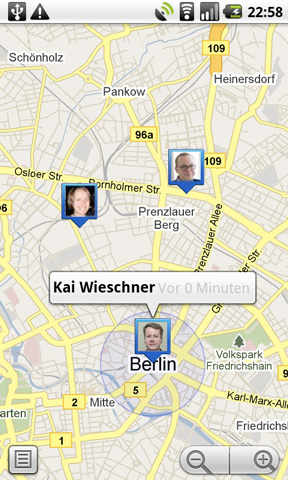
\includegraphics[ height=.10\paperheight]{images/latitude-see.jpg}
%	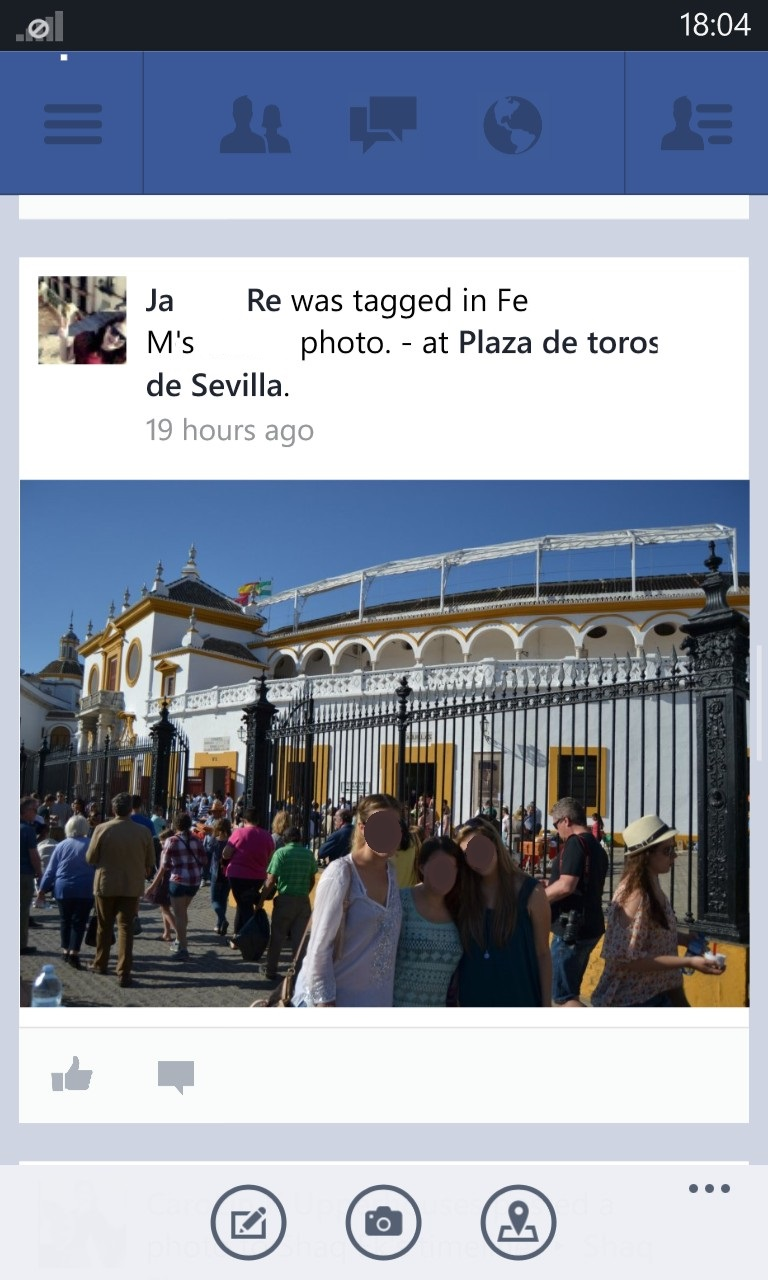
\includegraphics[ height=.10\paperheight]{images/facebook.jpg}
%\end{figure}

The application of this bachelor thesis should perform as a central information provider which combines the listed objectives and displays the daily activities of the smartphone. Those information will be presented in various ways and can be filtered by different criteria within a clear, intuitive graphical user interface.